\pdfoutput=1
\documentclass[11pt]{article}

\usepackage{acl}
\usepackage{times}
\usepackage{latexsym}
\usepackage[T1]{fontenc}
\usepackage[utf8]{inputenc}
\usepackage{microtype}
\usepackage{graphicx}
\usepackage{float}
\usepackage{titlesec}
\graphicspath{./images/}

\titlespacing*{\subsubsection}
{0pt}{5.5ex plus 1ex minus .2ex}{4.3ex plus .2ex}

\title{Playlist Generation using Emotion Recognition and Semantic Textual Similarity}

\author{
    Daniel King \\
    \And
    Thomas Hayter \\
}
\begin{document}
\maketitle


\section{Introduction}

Similarly to the proposal, try to convince your reader that your project is interesting. Introduce and motivate your problem. Discuss the formulation of your task.

\section{Related Work}
Short reports do not necessarily need a dedicated related work section; if you are running out of space, you can at least cover relevant work briefly, for example when substantiating your motivations or conclusions.


\section{Methodology}
The methodology of the project can be split up into different steps, which can be seen in the flowchart below. Each of the different steps will be explored in detail.

\begin{figure}[H]
    \centering
    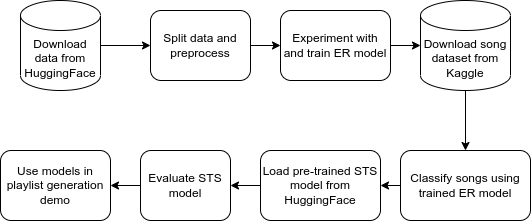
\includegraphics[width=0.48\textwidth]{images/codeFlow.png}
    \caption{Flow chart showing the steps of the project}
\end{figure}

\subsection{Emotion Recognition Model}
The first task to be performed was to train ane motion recognition model to classify a given input of text into an emotion class. The dataset used was the dair-ai/emotion dataset \cite{emotiondata} from HuggingFace. The dataset consists sentences that have been classified into one of six separate emotion classes - sadness, joy, love, anger, fear and surprise. The dataset contains two separate splits; one with 20,000 samples split into a training, testing and validation set, and another with 417,000 samples in one set. For this project, the larger split with 417,000 samples was chosen to train the model.

After being read in, the dataset was checked for imbalances between the labels in the dataset, which was immediately obviously present. The sadness and joy classes had 121,187 and 141,067 samples respectively, whils the surprise class only have 14,972 samples. To combat this imbalance, downsampling was performed to randomly select 5,000 samples from each of the classes to form a new dataset of 30,000 samples. Due to a lack of dedicated hardware to quickly train models, a smaller dataset of only 2,000 samples was created using the same downsampling method - to be used for experimenting with hyperparameters before training the final model. The larger dataset was split into a training and testing set, with a 0.85:0.15 train:test split; resulting in 25,500 samples being used for training and 4,500 for testing. The smaller dataset was also split.

The approach decided upon to create the model was to fine-tune a pre-trained BERT \cite{bert} model, by minimising cross entropy loss on the predictions of the classes. This was done using PyTorch and transformers. To preprocess the data, all of the data was encoded using the BertTokeniser, which tokenised the data, then returned both the input ids of all of the tokens, as well as the attention mask for the given input, so that padded values can be ignored (padding was used to ensure all inputs were of the same length). Before tuning the final model, an experiment was run with different model parameters to see which gave the best performance, and this experimentation will be discussed in more detail in the evaluation section. Using the best found parameters, the model was then fine-tuned on the larger training set by minimising cross entropy loss. The model returns logits, so an argmax function was used to get the predicted class from the output of the model. Metrics such as the precision, recall and f1 score across the different classes were calculated. The final trained model was then saved using PyTorch to be loaded in later when making predictions.

\subsubsection{Generating Song-Emotion Dataset}
To have songs to generate playlists from, the Spotify Million song dataset \cite{spotify} from kaggle was used. The dataset consists of songs with the artist, song title, a link to the song and song lyrics. To create the emotion-song dataset, the lyrics of the songs are first cleaned to remove newline characters, then passed into the trained emotion recognition model. The logits from the output of the model were taken, and any class with positive logits returned was said to be an emotion 'present' in the current song lyrics. Using this output of the emotion classes for each song, a dictionary of emotions mapping to a list of indices of the songs containing the emotions was constructed to be used alongside the song dataset in the final demo.

\subsection{STS Model}

Evaluating the performance of the model on song data, a custom testing metric was written. Taking a random song from a given emotion class, two other songs were selected - one from the same emotion class, and another from a random differing emotion class. 
To calculate the semantic textual similarity between two songs, a MiniLM \cite{minilm} model, which is a distilled version of a large transformer model scuh as BERT \cite{bert} was used. The particular model in question had 6 layers, was finetuned on a dataset of 1B sentence pairs and was loaded from HuggingFace \cite{stsmodel} using sentence-transformers. To compare the similarity between embeddings generated between by this model, a function to compute cosine similarity was written and used. All pre-processing/encoding needed was performed by the model itself, so no such code was necessary when using this model. 
An experiment to evaluate the performance of this model was written and run, but shall be discussed in the evaluation section of this report.

\subsection{Demo}
\begin{figure}[H]
    \centering
    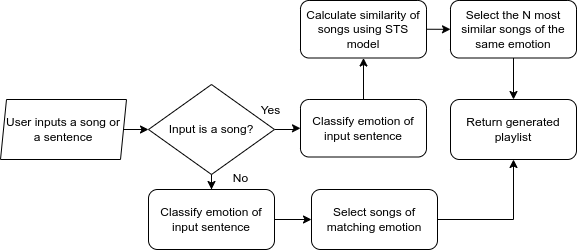
\includegraphics[width=0.48\textwidth]{images/DemoFlow.png}
    \caption{Flow chart showing the program flow of the demo}
\end{figure}

The flow chart in Figure 2 depicts the code flow of the final demo notebook. Both the ER model and the STS model are loaded into the notebook, as well as the song dataset and the song-emotion dictionary. The user is allowed to generate playlists in two different ways. First, they can enter an input sentence, which will have its emotion detected by the ER model, and then a playlist, of length defined by the user, with songs of the same emotion as the input sentence will be generated. The second option is to input song lyrics. In this option, the emotion of the song is detected and songs from the same emotion are selected as candidates for the playlist. Then, the STS model calculates the similarity between the input lyrics and the songs in the database, and the top N most similar songs are selected to be put into the playlist - where N is the length of the playlist defined by the user.

\section{Evaluation}
Similarly, describe your experimental setup and what you are trying to demonstrate with the experiment, and your expectations. Try to formulate a hypothesis such as ``By doing X, we expect Y to happen, because … . If Y does not happen, then it means Z, because...''. Present the results of your experiments and show how they support or contradict your hypothesis in a coherent manner, making use of graphs and tables as necessary. 

\section{Discussion}
The results you obtained should be analysed, interpreted and discussed. Do they correspond to what you have expected? Are they surprising or unexpected? Try to find an explanation for what you have observed, but be careful about making statements that are too strong or too general. Are your explanations substantiated by your experimental evidence? How do your results relate to what others have done? This is another point in the report where you could link back to existing literature, especially when comparing your results with those obtained in previous work. Depending on the depth of the discussion, this can be either its own section, or can be merged with the evaluation section.

\section{Conclusion}
Summarise what you have done to address the problem, and what it potentially means. What could be some reasonable follow-on work based on what you have done? 

\bibliographystyle{acl_natbib}
\bibliography{custom}


\end{document}
